\documentclass{aa}
\usepackage{txfonts}
\usepackage{amsmath}
\usepackage{booktabs}
\usepackage{bm}
\usepackage{graphicx}
\usepackage{hyperref}

\newcommand{\Msun}{M_\odot}
\newcommand{\Mst}{M_\star}
\newcommand{\dex}{\,\mathrm{dex}}

\begin{document}

\title{The observable dependence of correlated selection bias in JWST high-redshift galaxies}
\subtitle{A model-independent cross-depth measurement}

\author{S. Pandev\inst{1}}

\institute{Independent researcher, Santa Clara, CA, USA\\
  \email{stilianpandev@gmail.com}; ORCID: 0009-0005-8153-071X}

\titlerunning{Observable dependence of high-$z$ selection bias}
\authorrunning{S. Pandev}

\date{}

\abstract{%
The abundance of UV-bright and massive galaxies at $z\gtrsim8$ measured by JWST exceeds
pre-launch expectations. One candidate is a \emph{correlated} selection bias: the
noise that scatters a galaxy above the detection threshold is correlated with the noise on its
inferred properties, so a flux-selected sample is biased in a way forward-modelling removes
only under an assumed scatter model. We show that survey \emph{depth} is an exclusion
restriction---a variable that changes detection but not the true property---and use it to measure
this bias directly, with no scatter model, by comparing the same galaxies imaged to two depths.
In JADES~DR5, with per-tier SED refitting, the bias is strongly \emph{observable dependent}. For stellar mass it is small and \emph{negative}: a rest-UV selection
up-scatter makes the spectral energy distribution look younger and bluer, lowering the inferred
mass, so the high-$z$ stellar mass function is \emph{buffered} against this bias rather than
inflated by it. The measurement yields a coherent spectrum: near the detection limit galaxies are
biased towards younger ages, lower dust, and higher specific star-formation rate, while the UV
luminosity is biased strongly bright. The sign of the mass bias flips at the Balmer break, so
selection in a rest-optical band would instead \emph{inflate} the mass function. The sign
structure is robust across independent template families; the magnitude is template dependent.
These results constrain the role of correlated selection in the $z\gtrsim8$ excess and flag
concrete biases in high-$z$ specific-SFR and dust measurements near detection limits.}

\keywords{galaxies: high-redshift -- galaxies: luminosity function, mass function --
galaxies: statistics -- methods: statistical}

\maketitle

% =====================================================================
\section{Introduction}
\label{sec:intro}

JWST has established that UV-bright and massive galaxies are more abundant at $z\gtrsim8$ than
pre-launch models predicted \citep{Finkelstein2023,Labbe2023,Harikane2023,Donnan2023}, in extreme
cases straining the cosmic baryon budget under $\Lambda$CDM \citep{BoylanKolchin2023}, with the
surprise concentrated in the slow evolution of the bright end \citep{Finkelstein2024}. Whether
this reflects new astrophysics---elevated star-formation efficiency, bursty star formation, low
dust---or residual measurement effects remains open. The inferred high end of the mass and
luminosity functions is where a small upward scatter in an inferred property is amplified into a
large upward scatter in number density: the classical Eddington bias \citep{Eddington1913}. The
SED-inference step compounds this; assumptions about the star-formation history alone shift the
inferred $z\simeq10$ stellar-mass density by up to $0.75\dex$ \citep{Harvey2025}.

Two features make the high-$z$ case more than ordinary Eddington bias. First, galaxies are
selected on observed flux, not on the property of interest, so at fixed true property the
brightest objects are preferentially detected. Second, the photometric noise that promotes a
galaxy to detection is correlated with the noise on its inferred properties. The result is a
\emph{correlated} selection bias: selection and measurement errors are not independent, and the
high end is biased by an amount that depends on the selection strength. The community standard for
handling this is forward-modelling---inject synthetic galaxies with an assumed intrinsic
distribution and scatter, recover them, and fit the transfer function
\citep{Weaver2023,Davidzon2017}, increasingly jointly with the population and SED models
\citep{Leistedt2016,Alsing2024}. This removes the correlated bias only to the extent that the
assumed scatter model is correct; a mis-specified scatter leaves a residual that is invisible
within the same model. Even analyses that combine fields of different depth fold them into such a
model \citep{Tornotti2025}, treating the depth contrast as additional data under an assumed
selection function rather than as an identifying instrument. What is missing is a
test that does \emph{not} assume the scatter model.

We provide one, and use it to make a measurement. The sample-selection model of
\citet{Heckman1979} makes explicit the condition under which a selection correction is
identified without a functional form: an \emph{exclusion restriction}, a variable that enters
selection but not the outcome. High-redshift surveys contain a natural one---the spatial variation
of survey depth. Selection-aware abundance modelling is well established in astronomy, from
measurement-error and truncated-data regression \citep{Kelly2007,Mantz2019} to input/output
completeness \citep{Leethochawalit2022}; what is new here is the identifying device (depth as an
exclusion restriction) and the model-independent estimator it licenses. Crucially, applying that
estimator to \emph{real} two-depth JWST data---not to flux, but to the full set of SED-inferred
quantities---shows that the correlated selection bias is not a single number but an
\emph{observable-dependent} effect with a definite sign structure, and that its sign for the
stellar mass is the opposite of the naive expectation.

Sect.~\ref{sec:method} formalises the estimator. Sect.~\ref{sec:data} applies it to JADES~DR5
with per-tier SED refitting. Sect.~\ref{sec:results} presents the results: the negative,
buffered mass bias; the response spectrum across SED quantities; and its dependence on the
selection band. Sect.~\ref{sec:implications} gives the implications and a wide-area forecast, and
Sect.~\ref{sec:summary} concludes. We assume a flat $\Lambda$CDM cosmology with
$H_0=70\,\mathrm{km\,s^{-1}\,Mpc^{-1}}$, $\Omega_{\rm m}=0.3$, and AB magnitudes.

% =====================================================================
\section{Depth as an exclusion restriction}
\label{sec:method}

Let $q$ be an intrinsic galaxy property (e.g.\ $\log_{10}\Mst$) and $\hat q=q+e$ its inferred
value, with measurement error $e$. A galaxy is detected when a latent selection index
$s=\gamma_0+\gamma_1 q+u$ exceeds a threshold. The correlated selection bias is the statement
$\mathrm{corr}(u,e)=\rho\neq0$: the up-scatter that promotes detection is correlated with the
up-scatter in the inferred property. In the Heckman framework the selected-sample expectation is
\begin{equation}
\mathbb{E}[\hat q\mid\text{detected}]=q+\rho\,\sigma_e\,\lambda(s),
\label{eq:heckman}
\end{equation}
where $\lambda=\varphi/\Phi$ is the inverse Mills ratio, largest near the selection limit. The
correction is identified---separable from a genuine change in the abundance---only if a variable
moves $s$ (hence $\lambda$) without moving $q$: an exclusion restriction. Absent one, the
correction rests entirely on the assumed parametric form---the same fragility as forward-modelling.

Survey depth is such a variable. Deeper imaging changes the detection probability at fixed $q$ but
not $q$ itself. This licenses a model-independent estimator. Consider the same galaxies imaged at
two depths, ``deep'' and ``medium.'' For a galaxy detected in both, compare the property inferred
at each depth,
\begin{equation}
\Delta\hat q=\hat q_{\rm medium}-\hat q_{\rm deep}.
\label{eq:matched}
\end{equation}
The true property cancels object-by-object, so no scatter or completeness model enters. Under
$\rho=0$ the two differ only by independent noise and $\mathbb{E}[\Delta\hat q\mid\text{both
detected}]=0$. Under $\rho\neq0$, detection in the shallower tier conditions on a larger selection
up-scatter, so by Eq.~\eqref{eq:heckman} the difference is a depth-differential measurement of the
correlated bias,
\begin{equation}
\mathbb{E}[\Delta\hat q\mid\text{both detected}]
=\rho\big[\sigma_{\rm medium}\,\lambda(s_{\rm medium})-\sigma_{\rm deep}\,\lambda(s_{\rm deep})\big],
\label{eq:diff}
\end{equation}
nonzero because the shallower tier sits closer to the limit (larger $\lambda$) and has the larger
measurement scatter $\sigma$; its sign is that of $\rho$ and its amplitude grows towards the limit.
Because it pools all jointly detected objects and the common density field cancels in the
difference, this matched-overlap estimator is cosmic-variance immune and far more powerful at fixed
volume than a binned abundance ratio.

The estimator makes no reference to any physical model. Its one requirement is per-tier
measurements of $q$. For a directly-observed quantity (a broadband flux) these are immediate. For
a derived quantity---stellar mass, star-formation rate, dust---they require refitting the SED at
each depth, which we now do.

% =====================================================================
\section{Application to JADES DR5 with two-depth SED refitting}
\label{sec:data}

We use the public JADES~DR5 GOODS-S NIRCam photometric catalogue (EAZY \texttt{z\_peak}, per-band
circular-aperture fluxes and inverse-variance weight maps; \citealt{Eisenstein2023}). We select
$z\simeq7$--$9$ galaxies (\texttt{z\_peak}$\in[7,9)$, $P(z>7)>0.7$) detected above $5\sigma$ in
\texttt{F150W}, and split them at the median \texttt{F150W} weight into a deep and a medium tier
of the \emph{same sky}. The deep tier ($N=1397$) is the high-S/N reference. We realise the medium
tier by degrading each deep galaxy's photometry, band by band, to the medium-tier median depth
using the real weight ratio (a $1.78\times$ noise increase in \texttt{F150W}) with a single shared
noise draw, so that the detection-band up-scatter and the property up-scatter are the \emph{same}
event---the physical realisation of $\rho$.

We infer stellar mass and the other SED quantities with \textsc{eazy} \citep{Brammer2008} at fixed
\texttt{z\_peak}, using the FSPS \citep{Conroy2009} quiescent+star-forming template set and 13
bands (\texttt{F090W}--\texttt{F444W} plus ACS). Fixing the redshift isolates the property-inference
correlation from photometric-redshift scatter. Because the estimator uses only \emph{differences}
of $\log_{10}$ mass for the same galaxy at the same redshift, the per-object distance
normalisation cancels exactly, and the mass difference reduces to the change in the template
coefficient combination---validated against the full \textsc{eazy} stellar mass to a constant
offset (correlation $0.999$). We measure the matched-overlap shift of Eq.~\eqref{eq:matched} for
each SED quantity, averaged over 24--40 independent degradation draws.

To separate the correlated-selection term from the ordinary bias that noisier photometry imprints
on faint galaxies, we use a brightness-matched null: survival decided by an \emph{independent}
degradation draw of \texttt{F150W} at the same depth, not entering the SED fit. The null selects
the same brightness distribution but does not condition on the property-affecting noise, so the
difference (signal $-$ null) isolates the correlated-selection bias---the mass analogue of the
independent-band null used for fluxes.

% =====================================================================
\section{Results}
\label{sec:results}

\subsection{The correlated-selection mass bias is negative}
\label{sec:mass}

The matched-overlap shift in stellar mass, net of the brightness-matched null, is
\emph{negative}: $\langle\Delta\log_{10}\Mst\rangle=-0.019\pm0.003\dex$ averaged over the sample,
rising in amplitude towards the selection limit ($-0.039\dex$ for galaxies within $\sim\!1$ mag
of the medium limit, S/N$\,$5--6; consistent with zero, $-0.003\dex$, well above it). The
proximity dependence is the signature of a selection effect (Eq.~\ref{eq:heckman}); the sign is
opposite to the naive Eddington expectation.

The mechanism is direct. Correlating, per galaxy, the \texttt{F150W} flux deviation with the
inferred-mass deviation over many degradation draws gives a negative response,
$\mathrm{d}\log_{10}\Mst/\mathrm{d}\sigma_{\rm F150W}\simeq-0.08\dex$ per $1\sigma$ of
detection-band noise (median per-galaxy correlation $-0.12$). At $z\simeq8$, \texttt{F150W} is
rest-frame ultraviolet: a positive flux fluctuation makes the SED bluer and younger, lowering the
mass-to-light ratio and hence the inferred mass. Selection on such an up-scatter therefore biases
the inferred mass \emph{low}. The high-$z$ stellar mass function is, in this sense,
\emph{buffered} against correlated selection: the effect present in the UV luminosity does not
propagate into the mass with the same sign.

\subsection{A response spectrum across SED quantities}
\label{sec:spectrum}

The same two-depth fits yield every SED quantity, so we measure the response of each to a
detection-band fluctuation (Fig.~\ref{fig:spectrum}). Near the limit the inferred population is
pushed coherently towards \emph{younger, bluer, higher specific-SFR} solutions:

\begin{table}
\centering
\caption{Response of SED-inferred quantities to a $+1\sigma$ fluctuation of the \texttt{F150W}
detection band, from the JADES two-depth fits (no selection applied; errors are galaxy bootstrap).
sSFR is amplified from both ends; dust and mass are suppressed.}
\label{tab:spectrum}
\begin{tabular}{lc}
\toprule
quantity & response per $\sigma_{\rm F150W}$ \\
\midrule
specific SFR              & $+0.073\pm0.006\dex$ \\
recent-mass fraction (youth) & $+0.082\pm0.008\dex$ \\
star-formation rate       & $+0.003\pm0.002\dex$ \\
stellar mass              & $-0.070\pm0.005\dex$ \\
dust $A_V$                & $-0.053\pm0.003$ mag \\
UV luminosity (anchor)    & $+1$ by construction \\
\bottomrule
\end{tabular}
\end{table}

The pattern is one coherent shift, not six independent ones. A detection-band up-scatter is
interpreted by the fit as extra young-stellar light at fixed longer-wavelength flux: the
star-formation rate barely moves, but the population is read as younger (recent-mass fraction up),
less dust-attenuated ($A_V$ down), lower in mass-to-light (mass down), and hence higher in
specific SFR (up from both numerator and denominator). The recent-mass fraction and the specific
SFR are the most strongly biased quantities ($\gtrsim\!0.07\dex$ per $\sigma$); because the
specific SFR is a widely-used high-$z$ diagnostic, its bias is the most consequential. The small
star-formation-rate response is the least robust entry, being limited by the coarse SFR sampling of
a twelve-template basis; we therefore do not draw conclusions from it.

\begin{figure}
\centering
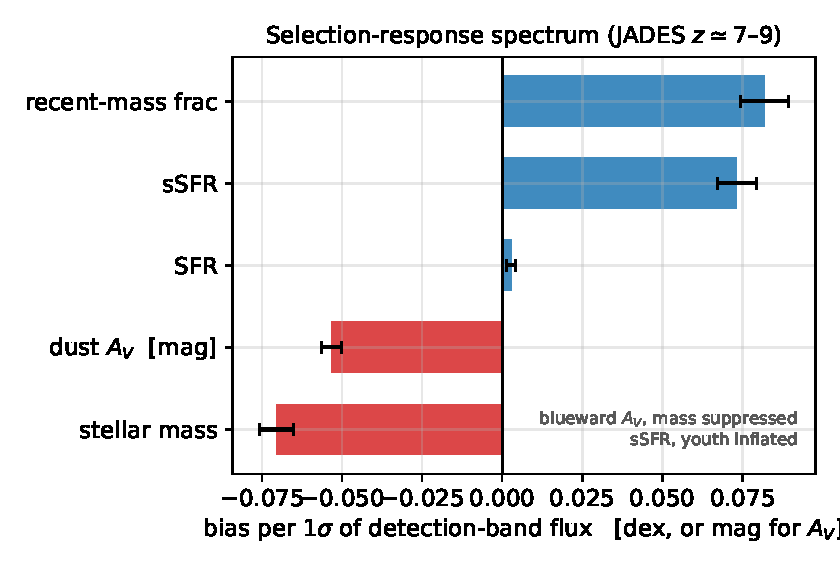
\includegraphics[width=\columnwidth]{figs/fig_spectrum.pdf}
\caption{Selection-response spectrum: the bias imprinted on each SED-inferred quantity by a
detection-band ($\texttt{F150W}$, rest-UV at $z\simeq8$) up-scatter, measured model-independently
from the JADES two-depth fits. Near a survey's detection limit galaxies are biased towards higher
specific SFR, younger ages, and lower dust, and towards \emph{lower} stellar mass; the UV
luminosity (the detection band itself) is biased bright. The near-limit bias is this response
times the mean up-scatter of the survivors.}
\label{fig:spectrum}
\end{figure}

\subsection{The sign is set by the selection band: a Balmer-break flip}
\label{sec:band}

Because the sign of the mass bias comes from what the detection band traces, it should depend on
the band's rest wavelength. We test this by regressing the inferred-mass deviation on the
independent noise of \emph{each} band simultaneously (a partial response per band).
Figure~\ref{fig:band} shows the result versus rest wavelength at $z\simeq8$. The mass response is
negative for every band blueward of the Balmer/$4000$\,\AA{} break---these trace young stars, so
an up-scatter lowers the inferred mass---and turns positive redward of it, reaching
$+0.37\dex$ per $\sigma$ in \texttt{F444W} (rest-frame optical continuum), which traces the
established stellar population. The response crosses zero at rest $\simeq4.3$--$4.4$\,k\AA, the
break itself.

The consequence is concrete: the sign of the correlated-selection mass bias is \emph{not
universal} but is set by the survey's selection band. A rest-UV--selected sample (JWST dropout
selection, as here) has its mass function buffered; a rest-optical-- or IRAC-selected sample would
have it \emph{inflated}. The sign structure is reproduced by an independent, data-driven template
family (Fig.~\ref{fig:band}, open symbols): the crossover wavelength and every sign agree, while
the magnitude shifts by tens of per cent---the sign is physical, the magnitude template dependent.

\begin{figure}
\centering
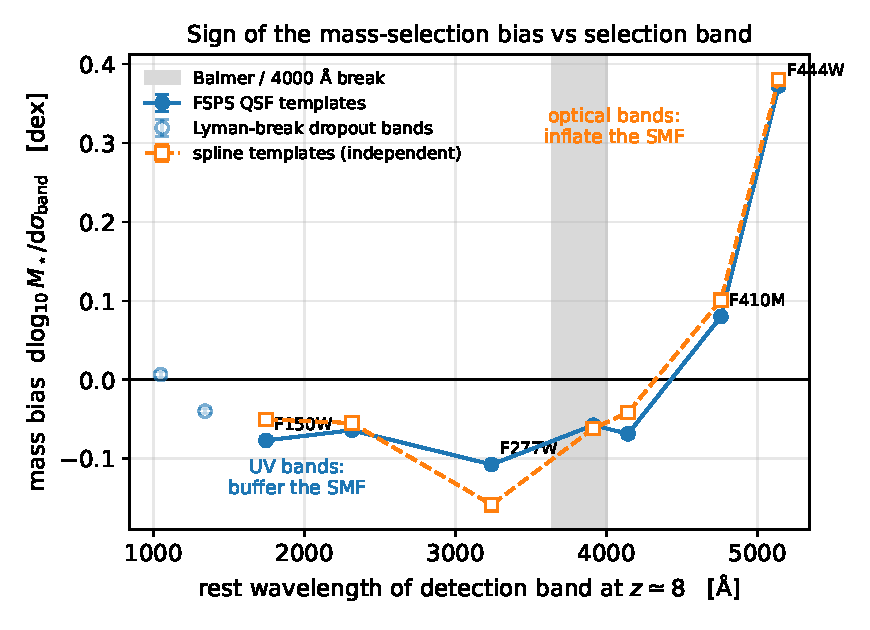
\includegraphics[width=\columnwidth]{figs/fig_band.pdf}
\caption{Correlated-selection bias of the stellar mass as a function of the \emph{rest wavelength}
of the detection band, at $z\simeq8$. Filled: FSPS quiescent+star-forming templates; open: an
independent data-driven template family. Bands blueward of the Balmer break (grey) buffer the mass
function (negative response); bands redward inflate it. The sign structure---and the zero crossing
at the break---is template independent; the amplitude is not. \texttt{F090W}/\texttt{F115W}
(Lyman-break dropout bands at $z\simeq8$) are shown but excluded from the crossover.}
\label{fig:band}
\end{figure}

\subsection{The contrasting positive case: UV luminosity}
\label{sec:uv}

Where the detection band \emph{is} the measured quantity, the bias is large and positive. Running
the same estimator on the \texttt{F150W} flux itself---which both selects and measures, so the
selection$\leftrightarrow$measurement correlation is physical and maximal ($\rho\simeq1$)---the
matched-overlap shift is a robust bright-ward boost ($8.7\sigma$; $-0.042$~mag overall, rising to
$-0.077$~mag at the medium limit), while an independently-degraded redder band shows no shift.
This is the UV-luminosity-function analogue of the mass measurement, with the opposite sign, and
confirms that the estimator recovers a strong bias where one is expected. The high-$z$ UV
luminosity function bright end thus carries a genuine depth-dependent selection boost that must be
removed before astrophysical interpretation---whereas the stellar mass function does not.

% =====================================================================
\section{Implications and forecast}
\label{sec:implications}

\paragraph{The $z\gtrsim8$ mass excess is not a correlated-selection artefact.} For UV/dropout-
selected samples the correlated-selection bias in stellar mass is small and of the wrong sign to
manufacture an excess of massive galaxies. This is a model-independent statement, made without a
scatter model, and it removes one specific systematic from the list of explanations for the
high-mass end---leaving genuine astrophysics (elevated efficiency, \citealt{Dekel2023}; bursty star
formation, \citealt{Sun2023,Shen2023}; low dust, \citealt{Ferrara2023,Cullen2024}) to be
distinguished by other means, such as galaxy clustering \citep{Munoz2023}.

\paragraph{Specific SFR and dust near detection limits are biased.} The response spectrum
(Table~\ref{tab:spectrum}) predicts that, near a survey's detection limit, inferred specific SFRs
are biased high and dust attenuations biased low, correlated with proximity to the limit. Both
biases point in the direction of the properties that have driven interest in early galaxies---high
specific SFR and burstiness \citep{Ciesla2024,Endsley2024} and unusually blue, dust-poor spectra
\citep{Topping2022,Cullen2024}---so a fraction of the most extreme near-limit values may be
correlated-selection artefacts rather than intrinsic. This is sharpened by the finding that bursty,
low H$\alpha$/UV signatures are several times more common among the UV-faintest galaxies
\citep{Endsley2024}, i.e.\ precisely the near-limit regime where this bias is largest. The effect is measurable, and correctable,
per survey from its own depth contrast.

\paragraph{Selection-band dependence for survey design and cross-survey comparison.} Because the
sign of the mass bias flips at the Balmer break (Fig.~\ref{fig:band}), mass functions from
rest-UV-- and rest-optical--selected surveys are biased in opposite directions. Comparisons that
mix selection bands---or that will select in rest-optical bands with \emph{Roman} and
\emph{Euclid}---should account for this; the two-depth estimator supplies the per-survey correction.

\paragraph{Forecast.} The matched-overlap estimator is cosmic-variance immune, so its precision is
set by the number of jointly-detected galaxies, i.e.\ by the \emph{overlap} area between depths.
Table~\ref{tab:fore} scales the JADES measurement to existing and planned two-depth data (with
order-of-magnitude overlap areas for the future surveys). A single JADES field already resolves the
mass bias at the few-hundredths-of-a-dex level; the wedding-cake deep/wide overlaps of \emph{Euclid}
and \emph{Roman} reach $\lesssim0.005\dex$, enough to map the
response spectrum as a function of mass, redshift, and selection band, and to probe the
$M_{\rm UV}\simeq-20$ bright end where the abundance excess is actually debated (and where, in a
wide-shallow survey, bright galaxies sit near the limit).

\begin{table}
\centering
\caption{Forecast $1\sigma$ precision on the matched-overlap property shift, scaling the JADES
measurement by $N_{\rm pair}^{-1/2}$ with overlap area. Cosmic variance cancels in the
difference, so overlap area---not total area---sets the precision.}
\label{tab:fore}
\begin{tabular}{lcc}
\toprule
two-depth data & overlap area & $\sigma(\Delta\log_{10}\Mst)$ \\
\midrule
JADES GOODS-S (this work)          & $0.03\,\mathrm{deg}^2$ & $0.003\dex$ \\
JADES GOODS-N$+$S                   & $0.06\,\mathrm{deg}^2$ & $0.002\dex$ \\
\emph{Euclid} Deep (deep/wide)     & $\sim\!5\,\mathrm{deg}^2$ & $\lesssim0.001\dex$ \\
\emph{Roman} HLTDS (deep/wide)     & $\sim\!1.5\,\mathrm{deg}^2$ & $\lesssim0.001\dex$ \\
\bottomrule
\end{tabular}
\end{table}

% =====================================================================
\section{Discussion}
\label{sec:discussion}

\paragraph{What is robust, and what is not.} The estimator is model-independent: it assumes no
scatter model and cancels the true property object-by-object. The \emph{sign} structure of the
response spectrum is physical---it follows from which stellar population each band traces---and we
find it reproduced across two independent template families with the zero crossing at the Balmer
break. The \emph{magnitudes} in Table~\ref{tab:spectrum} and Fig.~\ref{fig:band} depend on the SED
model (template set, star-formation-history and dust priors) at the tens-of-per-cent level, and we
quote them as such. All error bars in the text, tables, and figures are statistical (galaxy
bootstrap or realisation scatter); this SED-model systematic is larger and is the limiting
uncertainty on the magnitudes, though not on the signs. Two further choices are deliberate and bounded: we fix the redshift to isolate
the property-inference correlation from photometric-redshift scatter (a separate effect that a
floating-$z$ analysis would add), and we realise the medium tier by controlled degradation of the
deep photometry rather than from independently-observed shallow exposures, exactly as is standard
for depth-degradation tests; the real weight maps set the noise.

\paragraph{Relation to outshining and photometric-scatter studies.} The direction of the mass
bias---a detection-band up-scatter making the SED look younger, bluer and lower in mass---coincides
with the well-known outshining of old stellar populations by recent star formation, which biases
high-$z$ SED masses low \citep{Narayanan2023,GimenezArteaga2023,SorbaSawicki2018}, and with the
general sensitivity of inferred mass, age and dust to photometric noise. Those studies attribute the
effect to spatial resolution or to the assumed star-formation history; here it arises specifically
from proximity to the \emph{selection limit}, is measured model-independently from the depth
contrast rather than from mock recovery, and---the distinguishing feature---reverses sign with the
selection band, flipping at the Balmer break. The correlated-selection bias is therefore not a
restatement of outshining but a distinct, survey-dependent effect whose sign is set by that same
physics.

\paragraph{Relation to existing corrections and biases.} $1/V_{\rm max}$ \citep{PageCarrera2000}
removes the volume term but assumes $\rho=0$; forward-modelling removes the correlated term but only
under an assumed scatter model. The cross-depth estimator is complementary and assumption-light, using an exclusion
restriction already present in the data. The correlated selection is the SED-fitting cousin of the
Malmquist and Eddington \citep{Eddington1913} biases---and of the noise-correlated selection bias
already handled in weak-lensing shear calibration \citep{SheldonHuff2017}---and the collider
structure it induces
(conditioning on detection opens a spurious selection$\leftrightarrow$property association) places
it in the standard selection-bias framework of causal inference \citep{Hernan2004}. The same
depth-as-instrument construction applies wherever an observable-selected sample feeds an inferred
quantity---cluster mass--observable relations, photometric redshifts, and the UV-continuum-slope
measurements now used to argue for dust-free galaxies at $z>10$.

% =====================================================================
\section{Summary}
\label{sec:summary}

Survey depth is an exclusion restriction, and it turns the consistency of the same galaxies imaged
at two depths into a model-independent measurement of correlated selection bias---in \emph{any}
SED-inferred quantity, with no scatter model. Applied to JADES~DR5 with per-tier SED refitting,
this yields three results. (i)~The correlated-selection bias in stellar mass is small and
\emph{negative} for rest-UV--selected samples: a detection-band up-scatter makes the SED look
younger and bluer and lowers the inferred mass, so the high-$z$ stellar mass function is buffered,
not inflated---the $z\gtrsim8$ mass excess is not a correlated-selection artefact. (ii)~The bias
forms a coherent spectrum: near the detection limit galaxies are biased towards younger ages, lower
dust, and higher specific SFR, so a fraction of the most extreme near-limit values in these
quantities may be selection artefacts. (iii)~The sign of the mass bias flips at the Balmer break,
so it is set by the survey's selection band---rest-UV selection buffers the mass function,
rest-optical selection inflates it. The sign structure is template independent; the magnitude is
not. The estimator is cosmic-variance immune, and the deep/wide overlaps of \emph{Euclid} and
\emph{Roman} will map the full response spectrum and reach the bright end where the abundance
excess is debated.

% =====================================================================
\begin{acknowledgements}
This research made use of public data from the JWST Advanced Deep Extragalactic Survey (JADES),
obtained through the Mikulski Archive for Space Telescopes (MAST). It made use of \textsc{eazy},
\textsc{fsps}, \textsc{numpy}, \textsc{scipy}, \textsc{astropy}, and \textsc{matplotlib}. This
research received no specific grant from any funding agency, commercial or not-for-profit sector.
The author declares no conflicts of interest. Generative AI (a large language model) was used as an
assistive tool in code implementation, analysis, literature search, and manuscript editing; all
methods, results, and references were independently checked by the author, who takes full
responsibility for the content.
\end{acknowledgements}

% =====================================================================
\section*{Data Availability}
The observational data underlying this article are public: the JADES DR5 GOODS-S photometric
catalogue (JADES collaboration, via MAST). All analysis code---the two-depth SED-refitting
estimator, the response-spectrum and band-response measurements, and the figure scripts that
regenerate every number and figure---is available at \url{https://github.com/spsingularity/XDC}
and archived on Zenodo at \url{https://doi.org/10.5281/zenodo.21400942}.

\bibliographystyle{aa}
\bibliography{xdc}

\end{document}
